\documentclass{article}

\usepackage{PRIMEarxiv}

\usepackage[utf8]{inputenc} % allow utf-8 input
\usepackage[T1]{fontenc}    % use 8-bit T1 fonts
\usepackage[linktocpage=true]{hyperref}       % hyperlinks
\usepackage{url}            % simple URL typesetting
\usepackage{booktabs}       % professional-quality tables
\usepackage{amsfonts}       % blackboard math symbols
\usepackage{nicefrac}       % compact symbols for 1/2, etc.
\usepackage{microtype}      % microtypography
\usepackage{lipsum}
\usepackage{fancyhdr}       % header
\usepackage{graphicx}       % graphics
\graphicspath{{media/}}     % organize your images and other figures under media/ folder

% Packages added by Spencer
\usepackage{amsmath,amsthm,amssymb,scrextend}
\usepackage{appendix}
\AtBeginEnvironment{appendices}{\renewcommand\thesection{\Alph{section}}}
\usepackage{enumerate}
\usepackage{csquotes}
\usepackage{subcaption}
\usepackage{amssymb}
% \usepackage{bbm}
\usepackage[bb=pazo]{mathalpha}
\usepackage{bm}

\pagestyle{empty}
    
\newcommand\Bbbbone{%
  \ifdefined\mathbbb%
    \mathbbb{1}%
  \else%
    \boldsymbol{\mathbb{1}}%
  \fi}
  
\usepackage{xr}
\externaldocument{supplementary}
  
  
  

%%%%%%%%%%%%%%%%%%%%%%%%%%%%%%%%%%%%%
%%%%%%%%%%%%%%%%%%%%%%%%%%%%%%%%%%%%%

% \usepackage[pdftex]{graphicx}
% Standard, old-style thesis
% \usepackage{isutraditional}   
% \chaptertitle
% Old-style, thesis numbering down to subsubsection
\alternate
\usepackage{rotating}
% Bibliography without numbers or labels
\usepackage{natbib}
% Use the following line if you want square brackets and numbering system
%\usepackage[square, numbers]{natbib}

% this package is for getting certain math scripts like the 1 needed for an indicator function
\usepackage{bbm}

% using this package to make a better looking list
\usepackage{enumerate}
% try this one for a list as well. may be better
% \usepackage[font=itshape]{quoting}

% package for tables

\renewcommand{\bibfont}{\setstretch{1}\selectfont}
\setlength{\bibsep}{13.2pt}


\usepackage{chapterbib}
%\renewcommand\bibsection{\section*{\ref name}}
%\renewcommand\bibsection{\section*}
\renewcommand{\bibsection}{\section{References}}




%\bibliographystyle{apa}  % changed from apa, abbrv, unsrtnat
%\includeonly{titletoc,chapter1}
%Optional Package to add PDF bookmarks and hypertext links
% \usepackage[pdftex,hypertexnames=false,linktocpage=true]{hyperref}
\hypersetup{colorlinks=true,linkcolor=blue,anchorcolor=blue,citecolor=blue,filecolor=blue,urlcolor=blue,bookmarksnumbered=true,pdfview=FitB}

%\usepackage{titletoc}
% \usepackage{hyperref}
%%%%%%%%%%%%%%%%%%%%%%%%%%%%%%%%%%%%%
%%%%%%%%%%%%%%%%%%%%%%%%%%%%%%%%%%%%%

% Packages/commands added by Jarad
\usepackage{xcolor}
\newcommand{\jarad}[1]{{\color{red} Jarad: #1}}
\newcommand{\spencer}[1]{{\color{blue} Spencer: #1}}

%Header
\pagestyle{fancy}
\thispagestyle{empty}
\rhead{ \textit{ }} 

% Update your Headers here
\fancyhead[LO]{Bayesian nonlinear flu hospitalizations forecasting}
% \fancyhead[RE]{Firstauthor and Secondauthor} % Firstauthor et al. if more than 2 - must use \documentclass[twoside]{article}



  
%% Title
\title{Forecasting Influenza Hospitalizations Using a Bayesian Hierarchical Nonlinear Model with Discrepancy
%%%% Cite as
%%%% Update your official citation here when published 
% \thanks{\textit{\underline{Citation}}: 
% \textbf{Authors. Title. Pages.... DOI:000000/11111.}} 
}

\author{
  Spencer Wadsworth \\
  Iowa State University \\
  Ames, Iowa\\
  \texttt{sgw96@iastate.edu} \\
  %% examples of more authors
   \And
  Jarad Niemi \\
  Iowa State University \\
  Ames, Iowa\\
  \texttt{niemi@iastate.edu} \\
  %% \AND
  %% Coauthor \\
  %% Affiliation \\
  %% Address \\
  %% \texttt{email} \\
  %% \And
  %% Coauthor \\
  %% Affiliation \\
  %% Address \\
  %% \texttt{email} \\
  %% \And
  %% Coauthor \\
  %% Affiliation \\
  %% Address \\
  %% \texttt{email} \\
}

\begin{document} 

% \begin{appendices}
\section{FluSight forecast competition scoring results} \label{app:A_rwis}

In the CDC flu forecast competition, a baseline forecast was made to which all other forecasts were compared. The baseline forecast for a given state and week had as a median the most recent observed hospitalization count. The uncertainty was based on differences between previous hospitalizations, and is similar to the baseline forecast used in previous flu forecasting seasons and in the COVID-19 hub \cite[]{mathis2024evaluation, cramer2022evaluation}. 
The RWIS for one model was calculated by first taking the ratio of the average LWIS paired with every other model. This was then diveded by the same ratio for the baseline forecasts (see methods in \cite{mathis2024evaluation} for details, and see also the supplementary material).
 An RWIS less than 1 indicates the forecast outperformed the baseline forecast.
 Figures \ref{fig:rwis_ili_tile} and \ref{fig:rwis_hosp_tile} show the mean RWIS of hospitalization forecasts over all 24 models from section \ref{sec:analysis} for all locations and weeks of the 2023 flu season. Some similar patterns to those noted in section \ref{sec:analysis} emerge, including a slightly better performance by forecasts including discrepancy modeling over those which do not include discrepancy modeling and better overall performance by the SIR models than by the ASG forecast models. Interestingly, figure \ref{fig:rwis_hosp_tile} shows the LNORM model showing especially poor RWIS performance about three quarters into the season. This was not seen in the LWIS in figure \ref{fig:lwis_by_dist_loc}. 


\begin{figure}
    \centering
    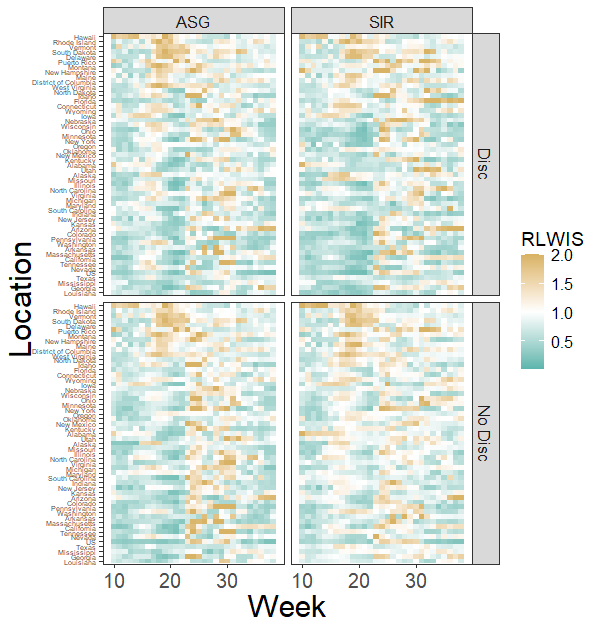
\includegraphics[scale=.7]{../../Images/rwis_ili_mod.png}
    \caption{RWIS averaged over all 24 models and horizons for forecasts across all locations and weeks. The plot is separated by the four ILI models. Dark blue is lower RWIS, and dark tan is higher RWIS where white is RWIS = 1}
    \label{fig:rwis_ili_tile}
\end{figure}


\begin{figure}
    \centering
    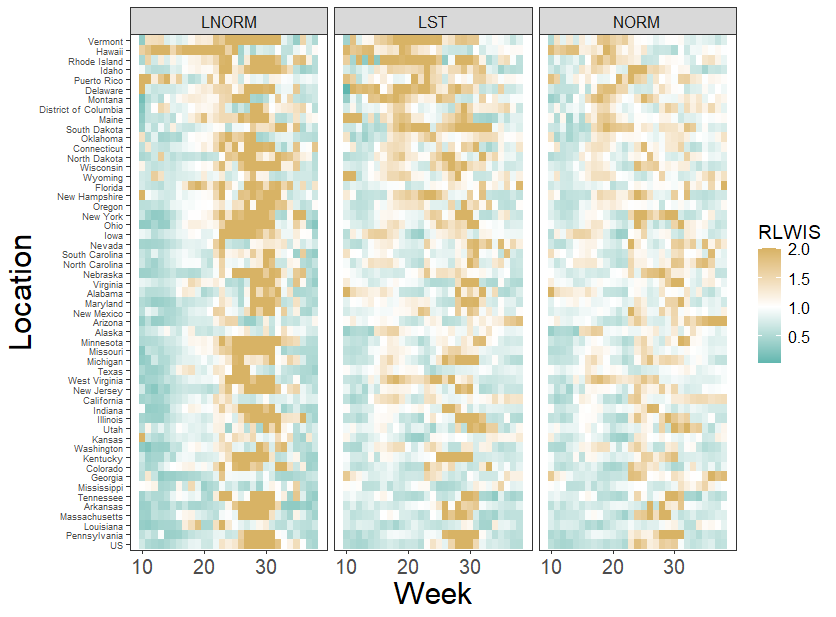
\includegraphics[scale=.6]{../../Images/rwis_hosp_mod.png}
    \caption{RWIS averaged over all 24 models and horizons for forecasts across all locations and weeks. The plot is separated by the three distribution choices for the hospitalization model. Dark blue is lower RWIS, and dark tan is higher RWIS where white is RWIS = 1}
    \label{fig:rwis_hosp_tile}
\end{figure}


Figure \ref{fig:state_median_points} shows the mean over weeks RWIS for the SIR and ASG forecast models with an RWIS less than 1 for the most locations. The plot on the left is from a forecast by an SIRD ILI model and a quadratic NORM hospitalization model. This forecast model had an RWIS less than 1 for 37 out of 53 locations. The plot on the right is from a forecast by an ASGD ILI model and linear NORM hospitalization model. This model had an RWIS less than 1 for 34 out of 53 locations.

\begin{figure}
\centering
\begin{subfigure}{.5\textwidth}
  \centering
  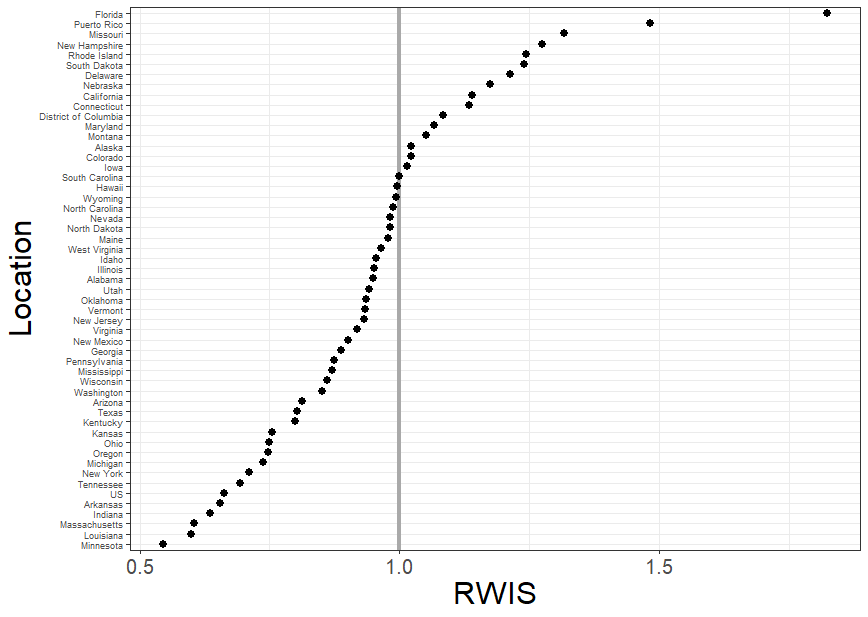
\includegraphics[width=1\linewidth]{../../Images/sir_disc_hosp_sq_ar1_rwis.png}
  % \caption{A subfigure}
  % \label{fig:sub1}
\end{subfigure}%
\begin{subfigure}{.5\textwidth}
  \centering
  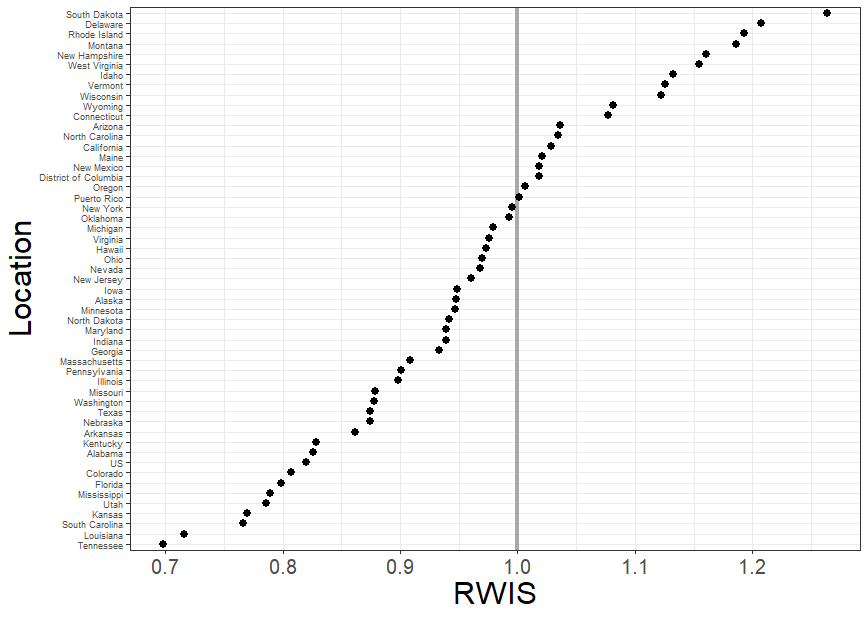
\includegraphics[width=1\linewidth]{../../Images/asg_disc_hosp_ar1_rwis.png}
  % \caption{A subfigure}
  % \label{fig:sub2}
\end{subfigure}
\caption{RWIS over the whole 2023 flu season for all 53 locations for hospitalization forecasts from an SIRD quadratic hospitalization model with normal errors (left) and forecasts from an ASGD linear hospitalization model with normal errors (right). An RWIS less than 1 (left of vertical grey line) indicates the model forecasts outperformed the baseline forecasts for that particular region.}
\label{fig:state_median_points}
\end{figure}






\section{Posterior distribution plots for select parameters}
\label{app:B_prior}

The figures in this section show 95\% credible intervals for model parameters under the several modeling schemes along with the prior distributions assigned to the parameters. Figure \ref{fig:posterior_theta_sir} is for parameters unique to the SIR ILI model. Figures \ref{fig:posterior_theta} and \ref{fig:posterior_zeta} are for parameters unique to the ASG models. Figure \ref{fig:sir_asg_shared} is for parameters shared by SIR and ASG models, including parameters used for modeling discrepancy. Figures \ref{fig:hosp_lin_params} and \ref{fig:hosp_nus_param} are for parameters used in hospitalization modeling.


\begin{figure}
    \centering
    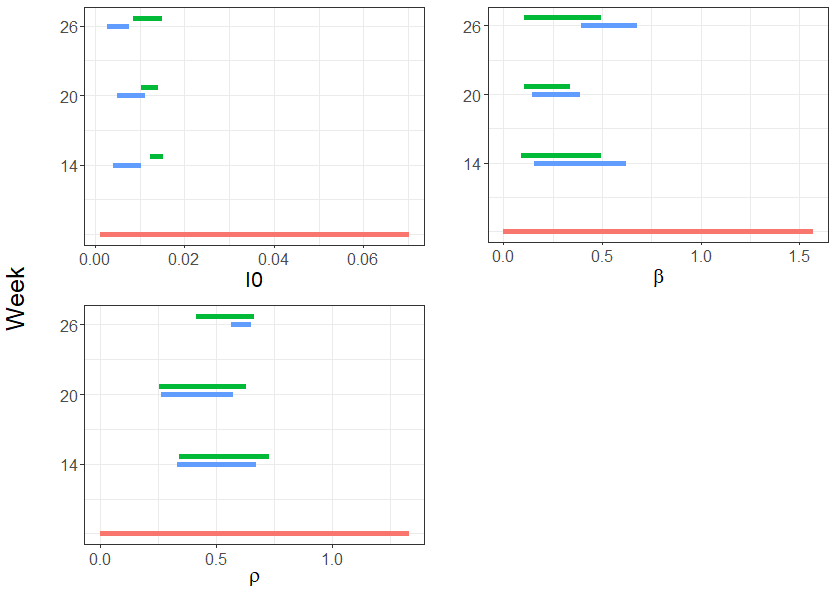
\includegraphics[scale=.6]{../../Images/posterior_theta_sir.png}
    \caption{Posterior 95\% credible intervals from ILI model for parameters of SIR differential equations. Shown are intervals from the US model of ILI for weeks 14, 20, and 26. The green is from the posterior where discrepancy is not modeled, and the blue is from the model where it is. The red interval is the 95\% interval of the prior distribution.}
    \label{fig:posterior_theta_sir}
\end{figure}

\begin{figure}
    \centering
    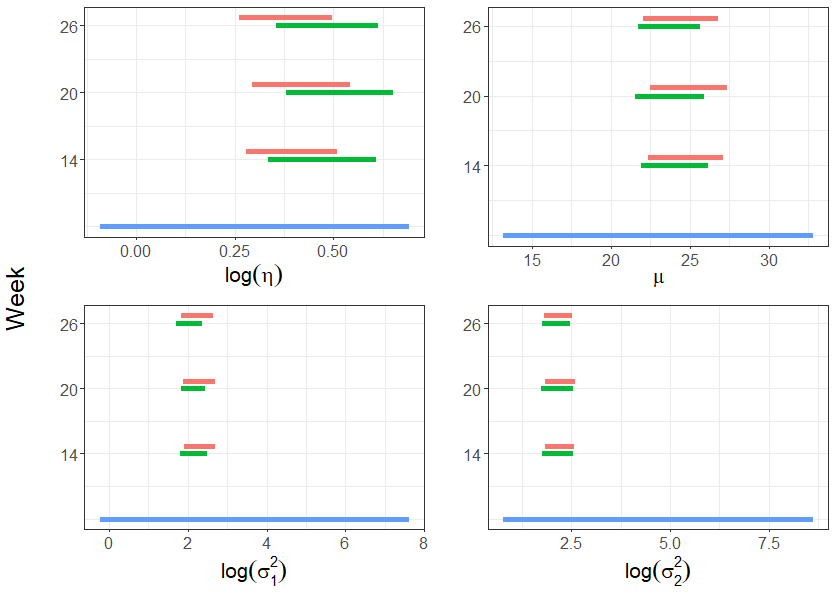
\includegraphics[scale=.6]{../../Images/posterior_theta.png}
    \caption{Posterior 95\% credible intervals from ILI model for parameters of ASG function. Shown are intervals from the US model of ILI for weeks 14, 20, and 26. The red is from the posterior where discrepancy is not modeled, and the green is from the model where it is. The blue interval is the 95\% interval of the prior distribution.}
    \label{fig:posterior_theta}
\end{figure}


\begin{figure}
    \centering
    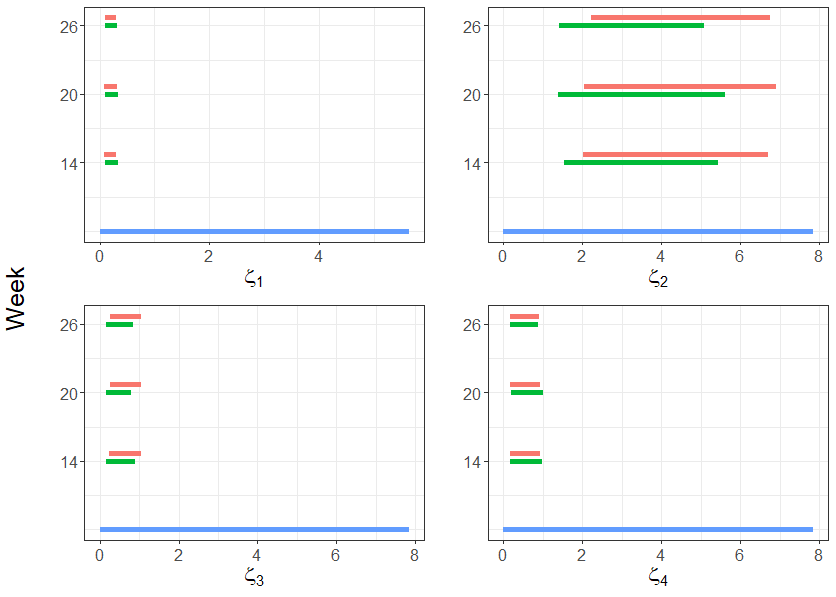
\includegraphics[scale=.6]{../../Images/posterior_zeta.png}
    \caption{Posterior 95\% credible intervals from ILI model for variance parameters of the ASG function. Shown are intervals from the US model of ILI for weeks 14, 20, and 26. The red is from the posterior where discrepancy is not modeled, and the green is from the model where it is. The blue interval is the 95\% interval of the prior distribution.}
    \label{fig:posterior_zeta}
\end{figure}

\begin{figure}
\centering
\begin{subfigure}{.5\textwidth}
  \centering
  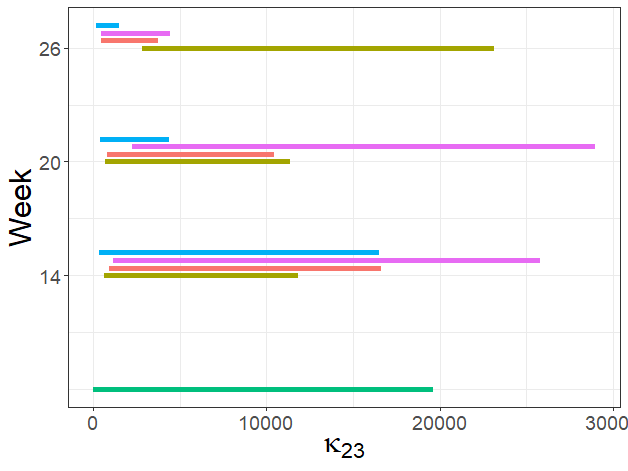
\includegraphics[width=.8\linewidth]{../../Images/posterior_kappa.png}
  % \caption{95\% posterior credible intervals from ILI model for scale parameter of the model distribution. Shown are intervals from the US model of ILI for weeks 14, 20, and 26. The blue is from the SIR model, purple from SIRD, red from ASG and yellow from ASGD. The green interval is the 95\% interval of the prior distribution.}
  % \label{fig:sub1}
\end{subfigure}%
\begin{subfigure}{.5\textwidth}
  \centering
  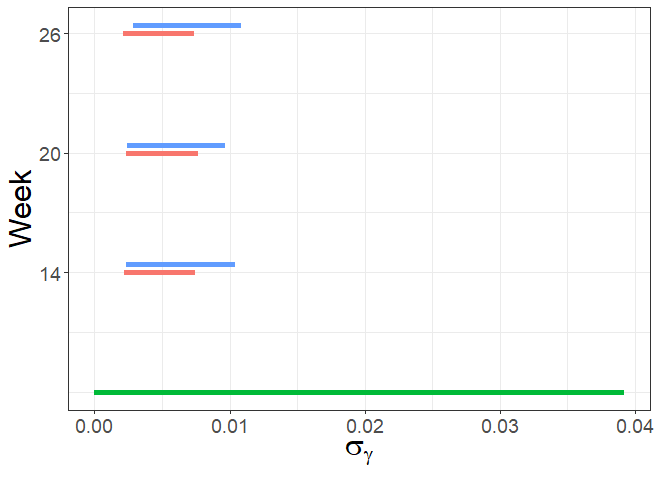
\includegraphics[width=.8\linewidth]{../../Images/posterior_sigma_gamma.png}
  % \caption{95\% posterior credible intervals from ILI model for scale parameter of modeled discrepancy. Shown are intervals from the US model of ILI for weeks 14, 20, and 26. The blue is from the SIRD model and red from ASGD. The green interval is the 95\% interval of the prior distribution.}
  % \label{fig:sub2}
\end{subfigure}
\caption{Posterior 95\% credible intervals from ILI model for scale parameter $\kappa_s$. Blue is from the SIR model, purple from SIRD, red from ASG and yellow from ASGD (left).  Posterior 95\% credible intervals from ILI model for scale parameter of modeled discrepancy $\sigma_{\gamma}$ (right). Shown are intervals from the US model of ILI for weeks 14, 20, and 26. Blue is from the SIRD model and red from ASGD. The green interval is the 95\% interval of the prior distribution.}
\label{fig:sir_asg_shared}
\end{figure}

\begin{figure}[hbt!]

\begin{subfigure}{.475\linewidth}
  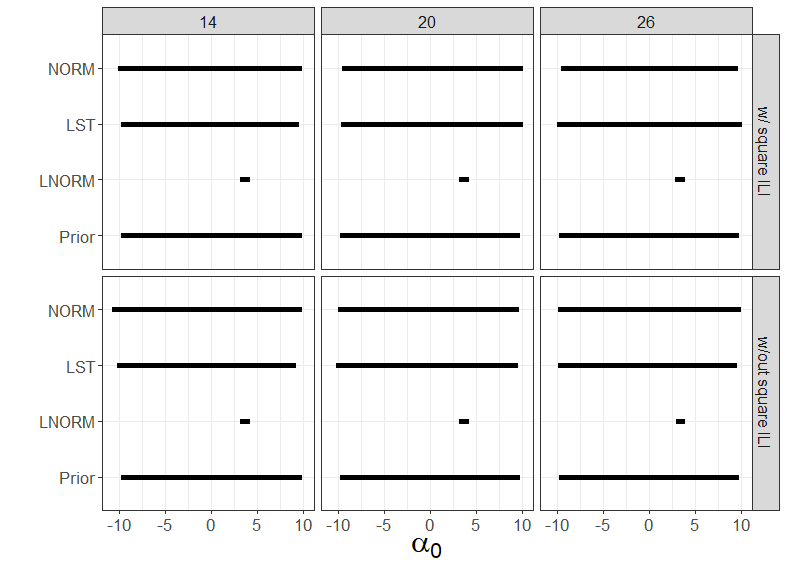
\includegraphics[width=\linewidth]{../../Images/alpha0_post.png}
  % \caption{}
  % \label{MLEDdet}
\end{subfigure}\hfill % <-- "\hfill"
\begin{subfigure}{.475\linewidth}
  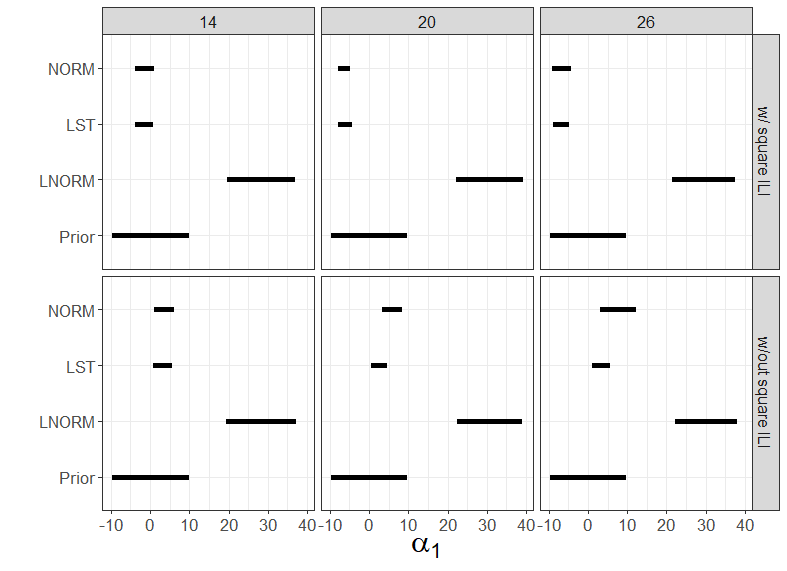
\includegraphics[width=\linewidth]{../../Images/alpha1_post.png}
  % \caption{}
  % \label{energydetPSK}
\end{subfigure}

\medskip % create some *vertical* separation between the graphs
\begin{subfigure}{.475\linewidth}
  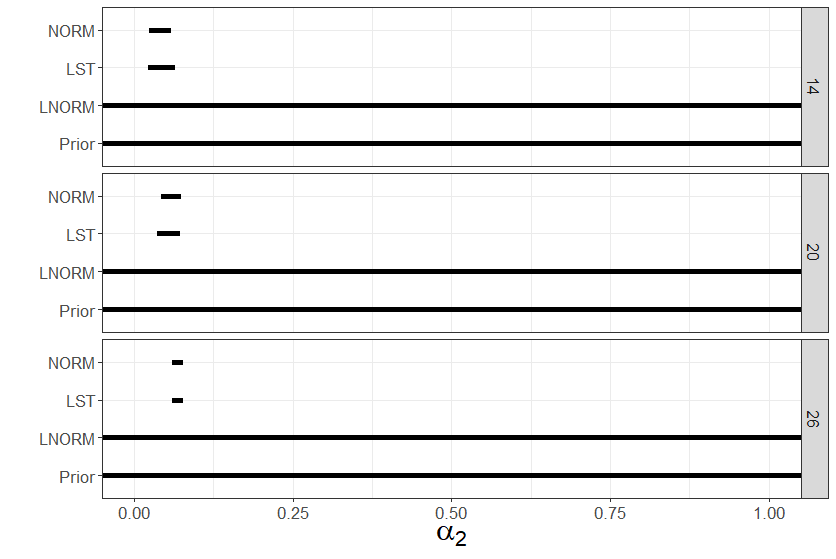
\includegraphics[width=\linewidth]{../../Images/alpha2_post.png}
  % \caption{}
  % \label{velcomp}
\end{subfigure}\hfill % <-- "\hfill"
\begin{subfigure}{.475\linewidth}
  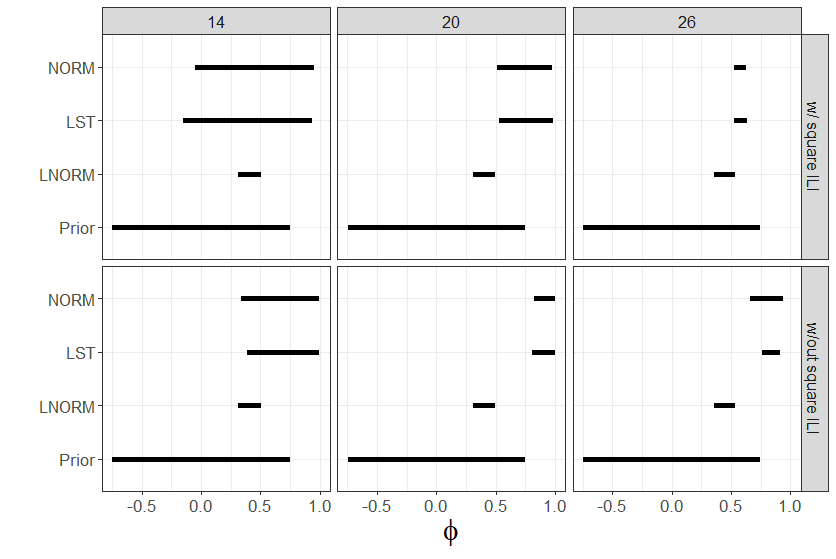
\includegraphics[width=\linewidth]{../../Images/phi_post.png}
  % \caption{}
  % \label{estcomp}
\end{subfigure}

\caption{Posterior 95\% credible intervals for $\alpha_0$ for the three hospitalization models separated by whether or not the squared ILI term was included. Intervals are for the US hospitalizations and weeks 14, 20 and 26 are shown (top left). Prior distribution 95\% interval is also included.  95\% posterior credible intervals for $\alpha_1$ for the three hospitalization models separated by whether or not the squared ILI term was included. Intervals are for the US hospitalizations and weeks 14, 20 and 26 are shown (top right). Prior distribution 95\% interval is also included.
95\% posterior credible intervals for $\alpha_2$ for the three hospitalization models. Intervals are for the US hospitalizations and weeks 14, 20 and 26 are shown (bottom left). Prior distribution 95\% interval is also included. 
95\% posterior credible intervals for $\phi$ for the three hospitalization models separated by whether or not the squared ILI term was included (bottom right). Prior distribution 95\% interval is also included. In each plot intervals are for the US hospitalizations and weeks 14, 20 and 26 are shown.}
\label{fig:hosp_lin_params}
\end{figure}


\begin{figure}[hbt!]

\begin{subfigure}{.475\linewidth}
  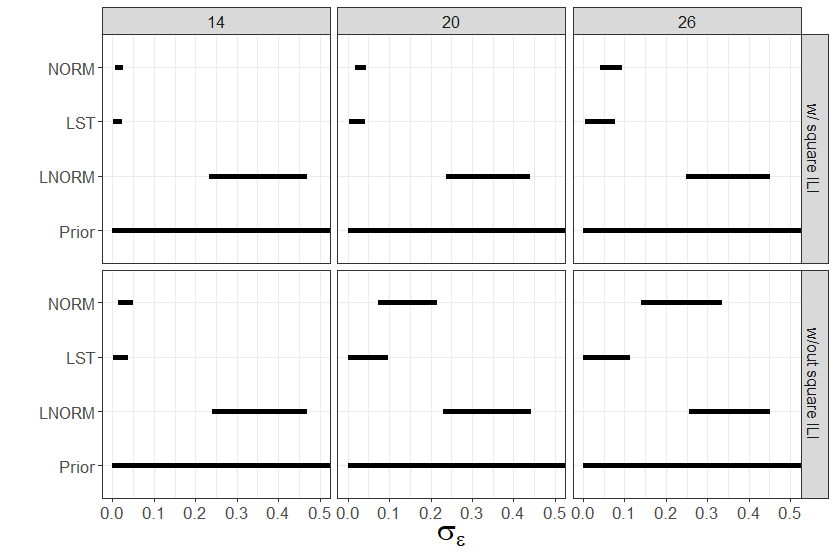
\includegraphics[width=\linewidth]{../../Images/sigma_epsilon_post.png}
  % \caption{}
  % \label{MLEDdet}
\end{subfigure}\hfill % <-- "\hfill"
\begin{subfigure}{.475\linewidth}
  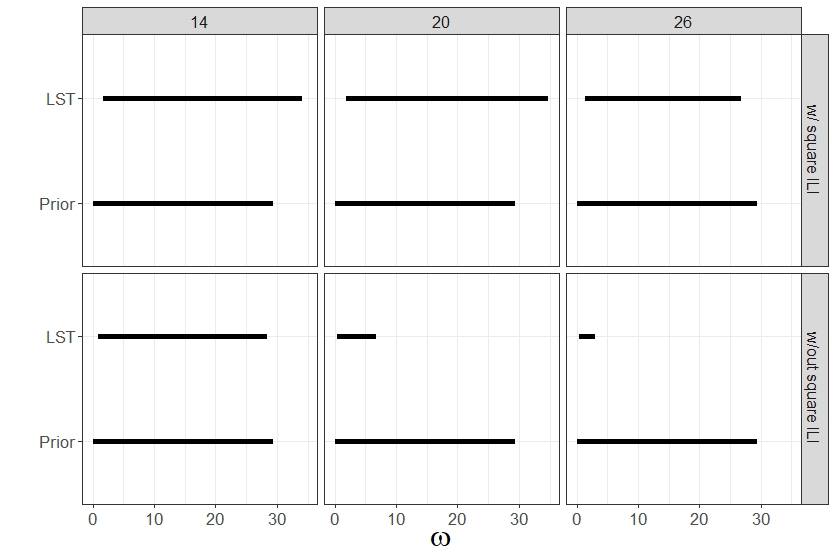
\includegraphics[width=\linewidth]{../../Images/omega_post.png}
  % \caption{}
  % \label{energydetPSK}
\end{subfigure}

\caption{Posterior 95\% credible intervals for $\sigma_{\epsilon}$ for hospitalization models with and without the ILI squared term. Intervals are for the US hospitalizations and weeks 14, 20 and 26 are shown (left). Prior distribution 95\% interval is also included.
95\% posterior credible intervals for $\omega$ for LST hospitalization models with and without the ILI squared term (right). Prior distribution 95\% interval is also included. In all plots intervals are for the US hospitalizations and weeks 14, 20 and 26 are shown.}
\label{fig:hosp_nus_param}
\end{figure}



% \end{appendices}

\end{document}